% !TEX root = ../notes_template.tex

\chapter{조화함수}

마지막 장에서는 다음 내용을 다룬다.

\begin{itemize}
\item[(1)] 라플라스 방정식이라 불리는 편미분방정식의 해가 되는 실함수로서 조화함수를 공부한다.
\item[(2)] 복소해석함수의 실수부와 허수부는 조화함수가 되며
국소적으로 역도 성립한다. 단순연결 영역에서는 전체적으로 역이 성립한다.
\item[(3)] 조화함수와 복소해석함수의 상호관계로부터 도출되는 결과들, 특히
디리클레 방정식이라 불리는 경계값문제에 대한 결과를 살펴본다.
\end{itemize}

\section{조화함수란?}

\begin{salt_definition} \label{def-5-1}
$U$를 $\mathbb R^2$의 열린 부분집합이라고 하자.
함수 $u:U \to \mathbb R$가
$2$차까지의 도함수가 존재하고 연속이면서(줄여서 $u\in C^2$라 한다)
라플라스 방정식
\[
(\Delta u)(x,y) := \dfrac{\partial^2 u}{\partial x^2} (x,y) 
+ \dfrac{\partial^2 u}{\partial y^2} (x,y) = 0,
\quad
(x,y) \in U
\]
을 만족하면, {\bf 조화함수}(harmonic function)라고 한다.
\end{salt_definition}

\begin{salt_example}\label{example-5-1}
$U=\mathbb R^2$라 하자.
함수 $u: U\to \mathbb R$가 모든 $(x,y)\in \mathbb R^2$에서
$u(x,y) = x^2-y^2$로 주어지면,
\begin{align*}
 &\dfrac{\partial u}{\partial x} = 2x, \hphantom{-} \quad  \dfrac{\partial^2 u}{\partial x^2} = 2, \\
 &\dfrac{\partial u}{\partial y} = -2y, \quad   \dfrac{\partial^2 u}{\partial y^2} = -2
\end{align*}
이므로 $\dfrac{\partial^2 u}{\partial x^2} (x,y) 
+ \dfrac{\partial^2 u}{\partial y^2} (x,y) = 2-2=0$이다.
$\mathbb R^2$에서 $u\in C^2$이고 $\Delta u=0$이므로 $u$는 조화함수이다.
\hfill $\diamondsuit$
\end{salt_example}

물론 모든 함수가 조화함수는 아니다.

\begin{salt_example}\label{example-5-2}
$(x,y)\in \mathbb R^2$에서 $\tilde u(x,y) = x^2+y^2$으로 정의된 함수  $\tilde u$를 생각하면,
\[
\dfrac{\partial^2 \tilde u}{\partial x^2} (x,y) 
+ \dfrac{\partial^2 \tilde u}{\partial y^2} (x,y) = 2+2=4\ne 0.
\]
따라서 $\Delta \tilde u$는 $\mathbb R^2$의 모든 점에서 $0$이 되지 않기에
$\tilde u$는 $\mathbb R^2$의 어떤 열린 부분집합에서도 조화함수가 될 수 없다.
\hfill $\diamondsuit$
\end{salt_example}

\begin{salt_exercise}\label{ex-5-1}
다음 함수 $u$가 주어진 열린집합 $U$에서 조화함수임을 보여라.
\begin{itemize}
\item[(1)] $u(x,y) = \log (x^2+y^2)$, $U = \mathbb R^2\setminus \{(0,0)\}$
\item[(2)] $u(x,y) = e^x\sin y$, $U=\mathbb R^2$.
\end{itemize}
\end{salt_exercise}

\begin{salt_exercise}\label{ex-5-2}
열린집합 $U$에 정의된 모든 조화함수의 집합 $\Har(U)$는
점별 연산에 대하여 실벡터공간을 이룸을 보여라.
\end{salt_exercise}

\begin{salt_exercise}\label{ex-5-3}
두 조화함수의 점별 곱으로 만든 함수도 조화함수가 되는가?
\end{salt_exercise}

{\bf 왜 조화함수에 신경써야 하는가?}

조화함수는 라플라스 방정식을 만족하기 때문에 중요한데,
라플라스 방정식은 여러가지 이유 중 다음 두 가지 때문에 특히 중요하다.
\begin{itemize}
\item[(1)] 라플라스 방정식은 편미분방정식(PDE)의 3가지 유형 중에서 
타원형 방정식이라는 중요한 유형에 속한다.
\begin{center}
\begin{tabular}{ |c|c| } 
 \hline
PDE 유형 & 예 \\ \hline \hline
타원형 & 라플라스 방정식 
$\dfrac{\partial^2 u}{\partial x^2} 
+ \dfrac{\partial^2 u}{\partial y^2} =0$ \\[1ex] \hline
포물형 & 확산 방정식 $\dfrac{\partial u}{\partial t} 
+ \dfrac{\partial^2 u}{\partial x^2} =0$ \\[1ex] \hline
쌍곡형 & 파동 방정식 $\dfrac{\partial^2 u}{\partial t^2} 
- \dfrac{\partial^2 u}{\partial x^2} =0$ \\[0.5ex]
\hline
\end{tabular}
\end{center}
\item[(2)] 라플라스 방정식은 많은 응용분야에서 사용된다.
다음과 같이 물리학에서 사용되는 예를 살펴보자.
유체역학에서 유체흐름의 ``속도 포텐셜(velocity potential)''은
라플라스 방정식을 만족한다. 한편, 정전기학에서는
정전기 전위(electronic potential)가 라플라스 방정식을 만족한다.
라플라스 방정식은 확률과정(stochastic process)과도 중요한 연결고리를 갖는다.
아래에서 이를 간단히 알아보자.
열린 단위원판 $\mathbb D:= \{z\in \mathbb C\,:\, |z|<1\}$을 생각하자.
입자가 한점 $z\in\mathbb D$에서 브라운 운동을 따른다고 하자.
(예를 들면, 무작위 운동을 만드는 물분자에 의해 충격받는 물 속의
꽃가루를 생각하자.)
직관적으로 무작위 운동으로 언젠가는 입자가 $\mathbb D$의 경계 
$\mathbb T:= \{ z\in \mathbb C \,:\, |z|=1 \}$를 벗어난다.
$z$에서 출발한 입자가 처음으로 단위원 $\mathbb T$를 벗어나는 
점을 $\zeta_z$라고 하자. 그러면 확률변수 $\zeta_z$는 단위원 위에 표시된다.
그림 \ref{fig-5-1}을 참고하라.
\begin{figure}[h!]
\begin{center}
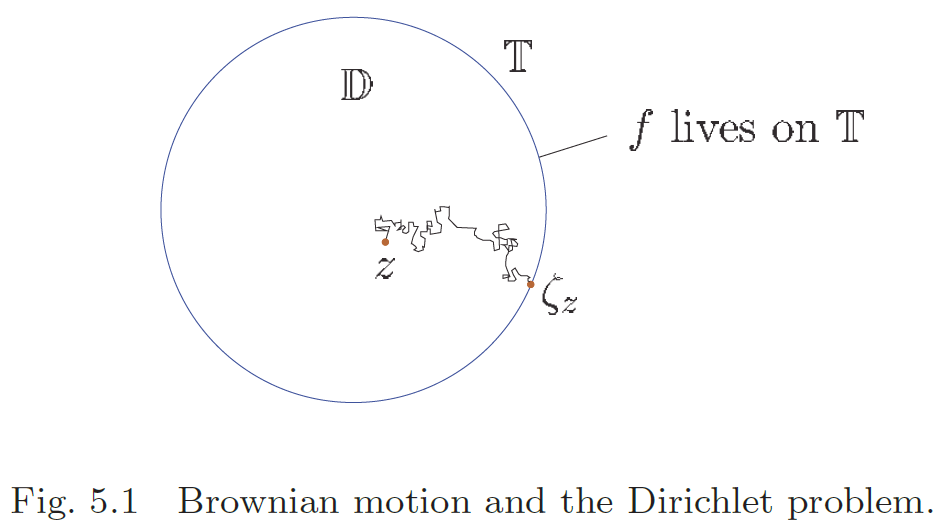
\includegraphics[width=0.6\textwidth]{./SaltChapter/fig-5-1}
\end{center}
\caption{브라운 운동과 디리클레 문제}
\label{fig-5-1}
\end{figure}
이제 연속함수 $f:\mathbb T \to \mathbb R$이 주어졌다고 하자.
그러면 $f(\zeta_z)$를 $\mathbb T$에 정의된 실수 값을 갖는 확률변수로 생각할 수 있다.
그 기댓값을 $\mathbb E(f(\zeta_z))$으로 표기하자.
이 값은 어디에서 출발하는지에 따라 달라진다. 즉, $z$에 의존하는 값이다.
$u:\mathbb D \to \mathbb R$을 $u(z) =\mathbb E(f(\zeta_z))$ ($z\in \mathbb D$)로 
정의하자. 이 때, $u$는 조화함수이고 실제로 디리클레 문제의 해가 됨이 알려져 있다.
이는 경계값 문제로 경계 $\mathbb T$에서 함수 $f:\mathbb T \to \mathbb R$가 
주어져 있을 때, $\mathbb T$의 내부 $\mathbb D$에서는 라플라스 방정식을 만족하고
경계 $\mathbb T$까지 연속함수로 확장되어 $f$와 일치하는 함수 $u$를 찾는 문제이다.
\[
\begin{cases}
\Delta u = 0, & \mathbb D\text{\,에서},\\
u\big|_{\mathbb T}= f.
\end{cases}
\]
\end{itemize}

\section{조화함수와 복소해석함수의 연결고리는 무엇인가?}

조화함수는 단지 실해석의 영역에 속해야 하는 것처럼 보일 수 있다.
이 절에서는 복소해석학에 대한 연구를 충분히 정당화할 수 있는 두가지 결과를 알아볼 것이다.
개략적으로 말하면, 열린집합에 정의된 조화함수는 국소적으로 복소해석함수의 실수부라는 
조건과 동치이다.

\begin{salt_theorem}\label{thm-5-1}
\
\begin{itemize}
\item[(1)] $U$가 $\mathbb C$의 열린 부분집합이고,
\item[(2)] $f:U\to \mathbb C$가 $U$에서 복소해석함수이면,
\end{itemize}
$\begin{cases}
u:= \Re(f), \\ v:= \Im(f)
\end{cases} \ $
는 $U$에서 조화함수이다.
\end{salt_theorem}

이 정리의 역도 참인데 다음과 같이 쓸 수 있다.

\begin{salt_theorem}\label{thm-5-2}
\
\begin{itemize}
\item[(1)] $U$가 단순연결영역이고,
\item[(2)] $u:U\to \mathbb R$가 $U$에서 조화함수이면,
\end{itemize}
$f:u+iv$가 $U$에서 복소해석함수가 되도록 하는
조화함수인 $v:U\to \mathbb R$가 존재한다.
\end{salt_theorem}

정리의 결론으로 얻은 함수 $f$는 $\Re(f)=u$와 $\Im(f)=v$를 만족한다.
따라서 정리에서 말하고자 하는 내용은  단순연결영역의 조화함수는 
어떤 복소해석함수의 실수부가 된다는 것이다.
단위원판은 단순연결영역이므로 단위원판의 모든 조화함수는 (적어도 정의된 단위원판에서는) 국소적으로
복소해석함수의 실수부가 된다.
단순연결영역의 조건이 불필요한 것이 아님을
연습문제 \ref{ex-5-5}에서 보게 될 것이다. 즉,
단순연결이 아닌 영역에 주어진 조화함수는 영역 전체에서 복소해석함수의 실수부로 표현되지 못할 수도 있다.
하지만 일단 미루고 첫번째 결과에 집중하도록 한다. 정리 \ref{thm-5-1}을 증명하기 전에
예제 \ref{example-5-1}을 다시 살펴보자.

\begin{salt_example}\label{example-5-3}
앞의 예제에서 $U = \mathbb R^2$이고
$u = x^2-y^2$이면,
$u= \Re(z^2) = \Re(x^2-y^2 + 2xy\,i)$이고 $z^2$은 전해석함수이다.
따라서 정리 \ref{thm-5-1}을 이용해도 $u$가  $\mathbb R^2$에서 조화함수임을
임을 알 수 있다.  실제로 정리 \ref{thm-5-1}로부터 $v:=2xy = \Im(z^2)$도 조화함수이다.
(물론 직접 계산하여 확인할 수도 있다.
\[
\dfrac{\partial v}{\partial x} = 2y, \quad  \dfrac{\partial^2 v}{\partial x^2} = 0, \quad
\dfrac{\partial v}{\partial y} = 2x, \quad   \dfrac{\partial^2 v}{\partial y^2} = 0
\]
이므로 $\dfrac{\partial^2 v}{\partial x^2}+ \dfrac{\partial^2 v}{\partial y^2} = 0$이다.)
%== [salt] 원문 수식에 오타 있음 (u-->v)

한편, 예제 \ref{example-5-2}와 정리 \ref{thm-5-1}로부터 
$\mathbb C$의 임의의 열린 부분집합 $U$에서 $\tilde u:= x^2+y^2$은 
복소해석함수의 실수부가 될 수 없다.
\hfill $\diamondsuit$
\end{salt_example}

{\bf 증명} (정리 \ref{thm-5-1})

$(x,y)\in U$에 대하여 $f(x+iy) = u(x,y) + iv(x,y)$로 쓸 수 있다.
$f$가 무한번 미분가능하므로, $u$, $v$는 모든 차수의 편미분이 존재하고
코시-리만 방정식에서
\begin{align*}
\dfrac{\partial^2 u}{\partial x^2} = \dfrac{\partial}{\partial x} \left( \dfrac{\partial u}{\partial x}\right)
\stackrel{\text{(C-R)}}{=} \dfrac{\partial}{\partial x} \left( \dfrac{\partial v}{\partial y}\right)
\stackrel{u\in C^2}{=} \dfrac{\partial}{\partial y} \left( \dfrac{\partial v}{\partial x}\right)
&\stackrel{\text{(C-R)}}{=} \dfrac{\partial}{\partial y} \left( - \dfrac{\partial u}{\partial y}\right) \\
&= - \dfrac{\partial^2 u}{\partial y^2}
\end{align*}
이므로 $u$는 조화함수이다. 유사한 방법으로
\begin{align*}
\dfrac{\partial^2 v}{\partial x^2} = \dfrac{\partial}{\partial x} \left( \dfrac{\partial v}{\partial x}\right)
\stackrel{\text{(C-R)}}{=} \dfrac{\partial}{\partial x} \left( - \dfrac{\partial u}{\partial y}\right)
\stackrel{v\in C^2}{=} \dfrac{\partial}{\partial y} \left( - \dfrac{\partial u}{\partial x}\right)
&\stackrel{\text{(C-R)}}{=} \dfrac{\partial}{\partial y} \left( - \dfrac{\partial v}{\partial y}\right) \\
&= - \dfrac{\partial^2 v}{\partial y^2}
\end{align*}
이므로 $v$도 조화함수이다. 
(다른 방법으로, $v= \Re(-if)$를 이용하여 증명할 수도 있다.)
\hfill $\square$

이제 열린 집합이 단순연결영역일 때 위의 결과의 역이 성립한다는 정리 \ref{thm-5-2}를 증명해보자.
앞에서 언급한 것처럼, 일반적인 영역에 대하여 조화함수는 영역 전체에 정의된
복소해석함수의 실수부로 쓸 수 없을 수도 있다. 연습문제 \ref{ex-5-5}의 예와 같이
\begin{align*}
\text{(1)\,} & U:=\mathbb R^2\setminus \{(0,0)\} \ (\text{단순연결영역이 아니다}) \\
\text{(2)\,} & u:= \log(x^2+y^2) \ (\text{$U$에서 조화함수이다})
\end{align*}
로 정하면, $U$에서 $u=\Re(f)$를 만족하고
$\mathbb C\setminus \{0\}$에 정의된 복소해석함수 $f$가 존재할 수 없다.

{\bf 증명} (정리 \ref{thm-5-2})

실수부가 $u$인 복소해석함수 $f$를 만들고
$v:=\Im(f)$가 조화함수임을 보이도록 하자.
우선 
\[
g=\dfrac{\partial u}{\partial x} - i \dfrac{\partial u}{\partial y}
\]
라 하자.
$g$가 복소해석함수임을 보이고 $g$의 부정적분을 만들면 우리가 원하는 $f$가 된다.
$g$가 복소해석함수임을 보이기 위해 정리 \ref{thm-2-2}를 사용한다.
우선  $u$가 조화함수이므로
\[
\Re(g) = \dfrac{\partial u}{\partial x}, \quad
\Im(g) = - \dfrac{\partial u}{\partial y}
\]
가 연속인 편도함수를 갖는다.
또한 $u$가 라플라스 방정식을 만족한다는 것을 이용하면
실수부와 허수부는 코시-리만 방정식을 만족함을 보일 수 있다.
\begin{align*}
\dfrac{\partial}{\partial x}(\Re(g)) 
&=  \dfrac{\partial}{\partial x}\left(\dfrac{\partial u}{\partial x} \right)
= \dfrac{\partial^2 u}{\partial x^2} = - \dfrac{\partial^2 u}{\partial y^2} 
=  \dfrac{\partial}{\partial y}\left(-\dfrac{\partial u}{\partial y} \right)
=  \dfrac{\partial}{\partial y}(\Im (g)) \\
\dfrac{\partial}{\partial y}(\Re(g)) 
&=  \dfrac{\partial}{\partial y}\left(\dfrac{\partial u}{\partial x} \right)
= \dfrac{\partial}{\partial x}\left(\dfrac{\partial u}{\partial y}\right)
= - \dfrac{\partial}{\partial x}  \left( - \dfrac{\partial u}{\partial y}\right)
=  - \dfrac{\partial}{\partial x}(\Im (g))
\end{align*}
따라서 $g$는 $U$에서 복소해석함수이다. 정리 \ref{thm-3-5}에 의하여
단순연결영역 $U$에서 부정적분 $G$를 갖는다.
$G=\tilde u + i\tilde v$를 실수부 $\tilde u$와 허수부 $\tilde v$로 나누어 보면
\begin{equation}\label{eq-5-1}
\dfrac{\partial u}{\partial x} - \dfrac{\partial u}{\partial y} = g = G'
= \dfrac{\partial \tilde u}{\partial x} + \dfrac{\partial \tilde v}{\partial x}
\end{equation}
이고
\[
\dfrac{\partial(u-\tilde u)}{\partial x} = 0
\]
적분학의 기본정리에 의하여 $u - \tilde u$는 국소적으로 수평방향을 따라 상수이다.
식 \eqref{eq-5-1}에 코시-리만 방정식을 적용하면
\[
- \dfrac{\partial u}{\partial y} = \dfrac{\partial \tilde v}{\partial x} 
\stackrel{\text{(C-R)}}{=} - \dfrac{\partial \tilde u}{\partial y}
\]
에서 
\[
\dfrac{\partial(u-\tilde u)}{\partial y} = 0
\]
이므로
$u-\tilde u$는 국소적으로 수직방뱡으로도 상수이다.
영역 $U$의 두 점은 계단형 경로로 연결가능하므로
$\tilde u-u$는 상수함수이다. 상수를 $C(\in \mathbb R)$라 하자.
그러면
\[
f:= G - C = (\tilde u-C) + i\tilde v = u + i\tilde v
\]
는 $U$에서 복소해석함수이며 $u=\Re(f)$와
$v:=\tilde v = \Im(G)$는 조화함수인 $f=u+iv$을 얻어 증명이 끝난다.
\hfill $\square$

\begin{salt_definition} \label{def-5-2}
열린집합 $U$에 정의된 조화함수 $u:U \to \mathbb R$에 대하여
$f:=u+iv$가 복소해석함수가 되는 조화함수 $v:U \to \mathbb R$를
$u$의 {\bf 조화켤레함수}(harmonic conjugate)라 한다.
\end{salt_definition}

\begin{salt_example}\label{example-5-4}
$v:=2xy$는 예제 \ref{example-5-1}에서 언급한 $u:=x^2-y^2$의 조화켤레함수이다.
왜냐하면, $z=x+iy$라 할 때,
\[
f:= u+iv = x^2-y^2 + 2xyi = (x+iy)^2 = z^2
\]
은 전해석함수가 된다.
\end{salt_example}

조화켤레함수에 상수를 더하면 새로운 조화켤레함수가 되므로 
조화켤레함수는 유일하지 않다.
정리 \ref{thm-5-2}는 단순연결영역에서 모든 조화함수가
조화켤레함수를 가진다는 것을 보장한다.
하지만, 조화켤레함수를 찾는데 특별히 유용하지는 않다.
(증명을 따른다면 부정적분 $G$를 직접 찾아야 하기 때문이다.)
좀 더 직접적인 방법은 다음 예제와 같이 코시-리만 방정식을 이용하는 것이다.

\begin{salt_example}\label{example-5-5}
$u=-(\sin x)(\sinh y)$라고 하자. 그러면,
\begin{align*}
\dfrac{\partial^2 u}{\partial x^2} &= + (\sin x)(\sinh y), \\
\dfrac{\partial^2 u}{\partial y^2} &= - (\sin x)(\sinh y)
\end{align*}
이므로 $u$는 $\mathbb R^2$에서 조화함수이다.
$\mathbb R^2$이 단순연결영역이므로 조화켤레함수가 존재함을 알 수 있다.
어떻게 찾을 수 있을까?
$v$가 조화켤레함수라면 $u+iv$가 복소해석함수이므로
$u$와 $v$는 코시-리만 방정식을 만족한다. 따라서 
\begin{align}
\dfrac{\partial v}{\partial x} &= -\dfrac{\partial u}{\partial y} = +(\sin x)(\cosh y),
\label{eq-5-2} \\
\dfrac{\partial v}{\partial y} &= \dfrac{\partial u}{\partial x} = -(\cos x)(\sinh y). 
\label{eq-5-3} 
\end{align}
식 \eqref{eq-5-2}에서 $y$를 고정하고 $x$에 대하여 적분하면
\begin{equation} \label{eq-5-4}
v = - (\cos x)(\cosh y) + C(y),
\end{equation}
여기서 상수 $C(y)$는 $y$에는 의존한다.
$C(y)$가 미분가능하다고 가정하면,
\[
- (\cos x)(\sinh y) \stackrel{\eqref{eq-5-3}}{=}
 \dfrac{\partial v}{\partial y} \stackrel{\eqref{eq-5-4}}{=}
=- (\cos x)(\sinh y)  + \dfrac{dC}{dy}(y).
\]
따라서
\[
\dfrac{dC}{dy}(y)=0
\]
이므로 $C(y)=C$이다. 
상수 $C$는 임의로 잡을 수 있는데 특별히 $C=0$으로 선택하자.
그러면 
\[
v = -(\cos x)(\cosh y)
\]
를 $u$의 조화켤레함수의 후보로 택할 수 있다.
이 선택이 맞는지 검증하기 위해 $u$, $v$가 코시-리만 방정식을 만족하는지 
빠르게 확인할 수 있어 $f:u+iv$는 복소해석함수이다.
한편, 연습문제 \ref{ex-1-37}을 계산을 활용하면
$f$가 복소해석함수임을 직접 확인할 수 있다.
\begin{align*}
f = u+iv &=  - (\sin x)(\sinh y) - i(\cos x)(\cosh y) \\
&= -i \left( (\cos x)(\cosh y) - i(\sin x)(\sinh y) \right)
= - i\cos z
\end{align*}
이므로 $f$는 전해석함수이다.
\hfill $\diamondsuit$
\end{salt_example}


\begin{salt_exercise}\label{ex-5-4}
다음 조화함수의 조화켤레함수를 찾아라.
\[
e^x\sin y, \quad x^3-3xy^2-2y, \quad x(1+2y).
\]
\end{salt_exercise}

\begin{salt_exercise}\label{ex-5-5}
$\mathbb C\setminus\{0\}$에 정의된 복소해석함수 $f$의
실수부가 $(x,y)\in \mathbb R^2 \setminus\{(0,0)\}$에서 $u(x,y) = \log(x^2+y^2)$이
될 수 없음을 보여라.\\
힌트: $v$를 $u$의 조화켤레함수라 하면, $h(z) := z^2\exp(-(u+iv))$는
복소해석함수이다. $|h|$를 찾고 $h'=0$임을 보여라.
$h'=0$로부터 $2/z$가 $\mathbb C\setminus\{0\}$에서 부정적분을 가지게 되는데
이는 불가능하다.
\end{salt_exercise}

\begin{salt_exercise}\label{ex-5-6}
\[
f (x+iy)= x^3+y^3 + iv(x,y),\quad (x,y)\in \mathbb R^2
\]
이 $\mathbb C$에서 복소해석함수가 되는 $v:\mathbb R^2 \to \mathbb R$를
찾을 수 있는가? 
\end{salt_exercise}

\section{(복소해석함수 $\leftrightarrow$ 조화함수)의 양방향성의 결과들}

앞에서 정리 \ref{thm-5-1}과 \ref{thm-5-2}의 결과로부터 조화함수의 실해석학 세계와
복소해석학 세계 사이의 유용한 상호 작용을 살펴보았다.

\begin{figure*}[h!]
\begin{center}
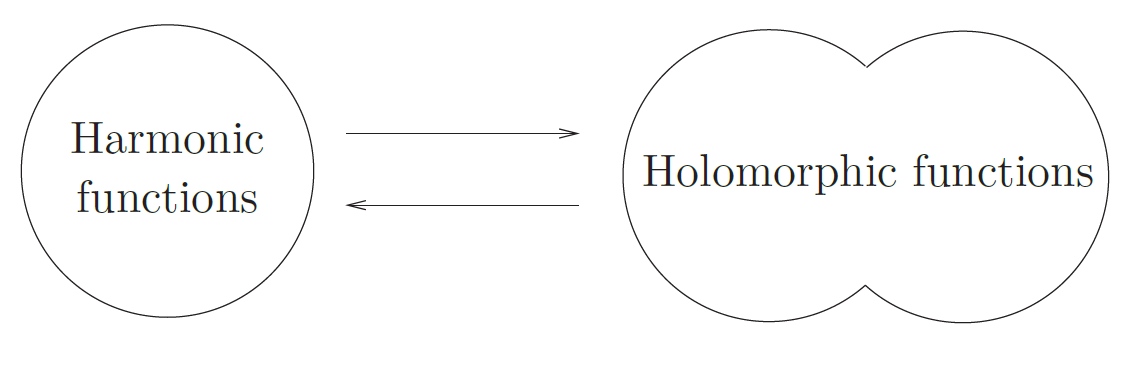
\includegraphics[width=0.7\textwidth]{./SaltChapter/fig-5-0-1}
\end{center}
%\caption{$\mathbb C$에 정의된 제곱급수의 수렴영역}
%\label{fig-4-0-3}
\end{figure*}

앞의 3개의 장에 걸쳐 복소해석함수가 갖는 많은 성질을 살펴보았다.
이제 이로부터 조화함수가 갖는 중요한 성질을 유도해보자.
특히, 다음 결과를 강조하고자 한다.
\begin{itemize}
\item[(1)] $u$가 조화함수이면 $C^\infty$
\item[(2)] 조화함수에 대한 평균값정리
\item[(3)] 조화함수의 최대원리
\item[(4)] 디리클레 방정식 해의 유일성
\end{itemize}

\subsection{매끄러운 조화함수}

\begin{salt_corollary}\label{coro-5-1}
조화함수는 무한번 미분가능하다.
\end{salt_corollary}

(조화함수의 정의는 단지 두번 미분가능한 성질만 요구한다.
그런데 라플라스 방정식을 만족한다는 성질로부터 무한번 미분가능하다는 놀라운 결과가 얻어진다.
이런 종류의 결과를 편미분방정식 이론에서 정칙성(regularity)이라 부른다.)

{\bf 증명}

$u$가 열린집합 $U$의 조화함수이고 $z_0=(x_0,y_0) \in U$라 하자.
그러면 $z_0$를 중심으로 반지름 $r$인 원판 $D$가 $U$에  포함되게 하는 $r>0$이 존재한다.
그런데 $u|_D$가 $D$에서 조화함수이고 $D$는 단순연결영역이다.
따라서 $D$에서 $\Re(f)=u$를 만족하는 복소해석함수 $f$가 존재한다.
$D$에서 $f$는 무한번 복소미분 가능한 함수이므로
$u$가 $D$에서, 특히 $z_0$에서 무한번 미분가능하다.
$z_0$의 선택을 임의로 할 수 있기 때문에 모든 점에서 무한번 미분가능하다.
\hfill $\square$

\begin{salt_exercise}\label{ex-5-7}
조화함수의 모든 편미분이 조화함수임을 보여라.
\end{salt_exercise}

\subsection{평균값 정리}

코시 적분공식을 이용하면
조화함수의 평균값 정리를 바로 얻을 수 있다.
어떤 점에서 조화함수는 그 점을 중심으로 하는 원에서의 함수값의 평균으로 주어진다.

\begin{salt_theorem} [조화함수의 평균값 정리] \label{thm-5-3}
\
\begin{itemize}
\item[(1)] $U$가 열린집합이고,
\item[(2)] $U$에서 $u:U\to\mathbb R$가 조화함수이고,
\item[(3)] $z_0\in U$,
\item[(4)] 원판 $\{ z\in\mathbb C\,:\, |z-z_0|<R \} \subset U$인 $R>0$이 존재하면,
\end{itemize}
모든 $r$ ($0<r<R$)에 대하여
$u(z_0) = \dfrac1{2\pi} \dint_0^{2\pi} u(z_0 + r\exp(it)dt$이다.
\end{salt_theorem}

{\bf 증명}

원판 $\{ z\in\mathbb C\,:\, |z-z_0|<R \} $이 단순연결영역이므로
$D$에서 실수부가 $u$인 복소해석함수 $f$가 존재한다.
한편, 코시 적분공식에 의하면, 
$C(t) = z_0 + r\exp(it)$ ($t\in[02\pi]$)로 주어진 원형경로 $C$애 대하여 
\begin{align*}
f(z_0) &= \dfrac1{2\pi i} \int_C \dfrac{f(z)}{z-z_0} dz
= \dfrac1{2\pi i} \int_C \dfrac{f(z_0+r\exp(it))}{r\exp(it)} ir\exp(it) dt\\
&= \dfrac1{2\pi} \int_0^{2\pi} f(z_0+r\exp(it)) dt.
\end{align*}
양변의 실수부만 취하면 원하는 결과를 얻는다.
\hfill $\square$

\subsection{최대원리}

최대절대값정리(\pageref{sec-4-6}페이지 참고)로부터 %== [salt] 페이지 인용방법은?
다음 정리를 얻는다.

\begin{salt_theorem} [최대원리] \label{thm-5-4}
\
\begin{itemize}
\item[(1)] $U$가 단순연결영역이고,
\item[(2)] $U$에서 $u:U\to\mathbb R$가 조화함수이고,
\item[(3)] $z_0\in U$가 모든 $z\in U$에 대하여 $u(z_0) \ge u(z)$를 만족하면,
\end{itemize}
$u$는 $U$에서 상수함수이다.
\end{salt_theorem}

{\bf 증명}

$u$를 실수부로 가지며 $U$에 정의된 복소해석함수 $f$가 존재한다.
그러면 $g(z)=\exp(f(z))$로 정의하면
$g:U\to\mathbb C$도 $U$에서 복소해석함수이다.
\[
|g(z_0)| = |\exp(f(z_0))| = e^{\Re(f(z_0))}
= e^{u(z_0)} \ge e^{u(z)} = |g(z)|
\quad (z\in U)
\]
최대절대값정리를 $g$에 적용하면
$g$는 $U$에서 상수함수이다.
그러면 $|g|$ 또한 $U$에서 상수, 즉, $|g| = e^{\Re(f)}$가 상수이다.
양변에 (실함수) 로그를 취하면 $u$는  $U$에서 상수함수이다.
\hfill $\square$

\section{디리클레 문제의 해의 유일성}

최대원리로부터 디리클레 문제의 해가 유일하다는 중요한 결론을 얻는다.
\begin{align*}
\mathbb D&:= \{ z\in\mathbb C\,:\, |z|<1\},\\
\mathbb T&:= \{ z\in\mathbb C\,:\, |z|=1\}
\end{align*}
라고 하자.

\begin{figure*}[h!]
\begin{center}
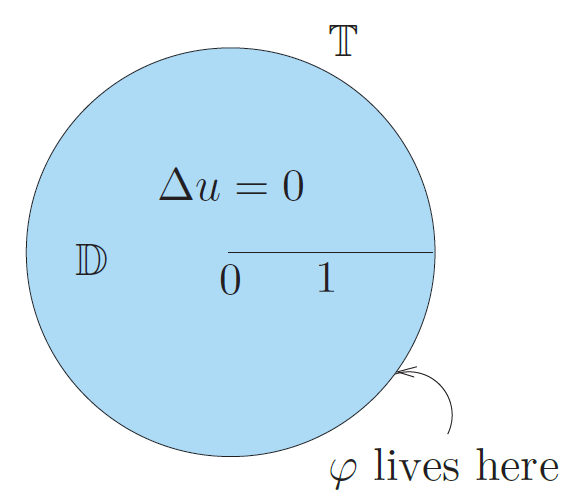
\includegraphics[width=0.4\textwidth]{./SaltChapter/fig-5-0-2}
\end{center}
%\caption{$\mathbb C$에 정의된 제곱급수의 수렴영역}
%\label{fig-4-0-3}
\end{figure*}

디리클레(Dirichlet) 문제는 다음과 같다.
\begin{quote}
주어진 연속함수 $\varphi: \mathbb T \to \mathbb R$에 대하여
\begin{itemize}
\item[(1)] $u$는 $\mathbb D \cup \mathbb T$에서 연속이고,
\item[(2)] $u|_{\mathbb T}=\varphi$,
\item[(3)] $u$는 $\mathbb D$에서 연속인 $2$차편도함수를 가지고,
\item[(4)] $\mathbb D$에서 $\Delta u  = 0$을 만족하는
\end{itemize}
$u: \mathbb D \cup \mathbb T \to \mathbb R$을 찾아라.
\end{quote}

주어진 함수 $\varphi$를 경계값이라고 부른다.
디리클레 문제를 푸는데 관심을 가지는 이유 중 하나는
열 전도, 정전기학, 유체역학 등의 응용에 필요하기 때문이다.
최대원리를 이용하면 다음 결과를 보일 수 있다.

\begin{salt_prop}\label{prpo-5-1}
디리클레 문제의 해는 유일하다.
\end{salt_prop}

{\bf 증명}

$u_1$, $u_2$가 경계값이 $\varphi$로 주어진 디리클레 문제의 
서로 다른 해라고 하자. 경계 $\mathbb T$에서는 $u_1 = u_2$이므로
$u_1$과 $u_2$는 $\mathbb D$ 내부의 어떤 점에서 다른 값을 가져야 한다.
그 점을 $w\in\mathbb D$라 하고 $u_1(w) > u_2(w)$라고 해도 일반성을 잃지 않는다.
그러면, $u:=u_1 - u_2$는 다음을 만족한다.
\begin{itemize}
\item[(1)] $u|_{\mathbb T}=0$,
\item[(2)] $u(w)>0$,
\item[(3)] $u$는 $\mathbb D$에서 조화함수이다.
\end{itemize}
$z_0\in \mathbb D\cup \mathbb T$를
콤팩트 집합 $ \mathbb D\cup \mathbb T$에서
실변수 연속함수인 $u$를 최대로 하는 점이라고 하자.
(1), (2)에서 $z\not\in \mathbb T$이므로
$z_0\in \mathbb D$이다.
그런데 최대원리에 의해 $u$는 $\mathbb D$에서 상수함수가 되어야 한다.
$u$는  $ \mathbb D\cup \mathbb T$에서 연속이므로
$\mathbb T$에서 $u$는 $0$이다.
따라서 $u$는  $ \mathbb D\cup \mathbb T$의 모든 점에서 $0$이 되어
가정 $u_1 = u_2$에 모순되어 증명이 끝난다.
\hfill  $\square$

\begin{salt_remark}\label{rem-5-1}
경계값이 $\varphi$로 주어진 디리클레 문제의 해는 
다음 포아송 적분공식(Poisson integral formula)으로 나타낼 수 있다.
\[
u(r\exp(it)) = \dfrac1{2\pi} \int_0^{2\pi} 
\dfrac{1-r^2}{1-2r\cos(\theta -t) + r^2} \varphi(\exp(i\theta))d\theta
\quad (\exp(i\theta) \in \mathbb T).
\]
코시 적분공식을 이용하면 이 공식을 유도할 수 있는데
약간의 계산 기술이 필요하여 여기서는 증명을 생략한다.
\end{salt_remark}

\begin{salt_exercise} [반평면에서의 디리클레 문제] \label{ex-5-8}
경계값으로  $b:\mathbb R \to \mathbb R$이 주어졌을 때,
닫힌 반평면 $y\ge0$에 정의된 연속 실함수로
$y>0$에서 조화함수이고, $h(x,0)=b(0)$를 만족하는 
$h$를 찾는 문제를 생각하자.
\begin{itemize}
\item[(1)] $b$가 다항식이면, $h(x,y) = \Re(p(x+iy))$로  $h$를 택하면 됨을 보여라.
\item[(2)] $b$가
\[
b(x) = \dfrac1{1+x^2}
\]
으로 주어지면, $(x,y) \mapsto \Re(b(x+iy))$는 해가 될 수 없다.
(왜냐하면, $z=i$에서 극을 갖기 때문이다.)
\[
h(x,y):= \Re\left(\dfrac{i}{z+i}\right) 
= \dfrac{y+1}{x^2+(y+1)^2}
\]
라 하면, 주어진 디리클레 문제의 해가 됨을 보여라.
\end{itemize}
\end{salt_exercise}

\begin{salt_exercise}\label{ex-5-9}
조화함수 $u:\mathbb R^2\to \mathbb R$가 모든 $(x,y)\in\mathbb R^2$에 대하여
$u(x,y)>0$를 만족한다면, $u$는 상수함수임을 보여라. \\
힌트: 실수부로 $u$를 가지는 전해석함수 $f$에 대하여  $\exp(-f)$를 생각해보자.
\end{salt_exercise}

\begin{salt_exercise}\label{ex-5-10}
라플라스 방정식의 정칙성이 항상 저절로 얻어지는 것은 아니다.
불연속함수가 라플라스 방정식을 만족하는 예를 소개해 보자.
$z\ne 0$에 대하여
$u:\mathbb R^2\to \mathbb R$를 $e^{-1/z^4}$의 실수부로 
원점에서는 $0$으로 정의하자.
\begin{itemize}
\item[(1)] $u$는 $0$에서 불연속임을 보여라.
\item[(2)] $u(x,0) = e^{-1/x^4}$, $u(0,y) = e^{-1/y^4}$임을 확인하라.
\item[(3)] $\mathbb C\setminus\{0\}$에 정의된 복소해석함수의 실수부로서
$u$는 $\mathbb R^2\setminus\{0,0)\}$에서 라플라스 방정식을 만족함은 이미 알고 있다.
\[
\dfrac{\partial^2 u}{\partial x^2}(0,0), \quad
\dfrac{\partial^2 u}{\partial y^2}(0,0)
\]
가 존재함을 보여라.
또한 $\dfrac{\partial^2 u}{\partial x^2}(0,0) + \dfrac{\partial^2 u}{\partial y^2}(0,0) =0$임을
증명하라.
\end{itemize}
\end{salt_exercise}

\begin{salt_exercise}\label{ex-5-11}
$D_1$, $D_2$가 $\mathbb C$의 영역이고
$\varphi: D_1 \to D_2$가 복소해석함수라고 하자.
$h:D_2\to \mathbb R$이 조화함수이면,
$h\circ \varphi : D_1 \to \mathbb R$도 조화함수임을 보여라.
이제 $\varphi: D_1 \to D_2$가 전단사 복소해석함수이고
역함수 $\varphi^{-1}: D_2 \to D_1$도 복소해석함수라고 가정하자.
이러한 함수를 {\bf 쌍정칙함수}(biholomorphism)라고 한다.
함수 $h:D_2\to \mathbb R$이 조화함수인 것은
$h\circ \varphi : D_1 \to \mathbb R$이 조화함수인 조건과 동치임을 보여라.

두 영역 사이에 쌍정칙함수가 존재하면
한 영역의 조화함수(복소해석함수도)를 다른 영역으로 옮길 수 있다.
$D_1$이 좋은 영역(반평면 또는 원판)이고 $D_2$가 복잡한 영역일 때
$D_2$의 문제(디리클레 문제와 같은)를 $D_1$의 문제로 바꾸고
$D_1$에서 해를 찾은 후 다시 $D_2$로 옮기는 것이 가능하다는 장점이 있다.

우선 주어진 영역 $D_1$과 $D_2$에 대하여
쌍정칙함수가 존재하는지에 대한 질문이 자연스럽다.
이 질문에 대한 답은 리만 사상 정리(Riemann mapping theorem)에서 주어진다.
증명은 이 책의 범위를 벗어나기 때문에 다루지 않으니
필요하면 [Conway(1978)]를 참고하라.


\begin{salt_theorem}[리만 사상 정리] \label{thm-5-5}
 단순연결영역 $D$가 $\mathbb C$의 진부분집합($D\ne \mathbb C$)이라고 하자.
 그러면 쌍정칙함수 $\varphi: D\to \mathbb D:=\{z\in\mathbb C\,:\, |z|<1\}$가
 존재한다.
\end{salt_theorem}

이 결과는 복소평면 전체가 아닌 임의의 두 단순연결영역 사이에
쌍정칙함수가 존재함을 보장한다. ($\mathbb D$를 통하여)
하지만, 실제로 쌍정칙함수를 찾는 알고리즘이 증명에 주어지는 것은 아니다.
$\mathbb H:= \{s\in\mathbb C\,:\, \Re(s) >0 \}$에 대하여
{\bf 뫼비우스(M\"obius) 변환} $\varphi: \mathbb H \to \mathbb D$
\[ 
\varphi(s) = \dfrac{s-1}{s+1},
\quad s\in \mathbb H
\]
은 우측 반평면 $\mathbb H$와 원판  $\mathbb D$사이의 쌍정칙함수임을 보여라.
\end{salt_exercise}

\section{참고}

연습문제 \ref{ex-5-5}, \ref{ex-5-6}, 그리고 정리 \ref{thm-5-2}는
[Beck, Marchesi, Pixton, Sabalka (2008)]에서 인용하였으며,
연습문제 \ref{ex-5-8}은 [Flanigna (1973)]을 기초로 만들어졌다.

